% !TEX program = xelatex
% 河海大学大学生创新创业训练项目成果
% DL-MPT(CoOp+ATP): 基于元任务微调与属性辅助推理的LVLM小样本学习
%
% 排版格式依据: 附件3.河海大学大学生创新创业计划项目研究报告以及论文排版格式
% 编译: xelatex → xelatex

\documentclass[10pt,a4paper]{ctexart}

% ==================== 页面设置 ====================
\usepackage[top=2.5cm, bottom=2.5cm, left=2.9cm, right=3.2cm]{geometry}
\usepackage{setspace}
\usepackage{fancyhdr}
\usepackage{titlesec}
\usepackage{graphicx}
\usepackage{float}
\usepackage{booktabs}
\usepackage{amsmath}
\usepackage{hyperref}
\usepackage{caption}
\usepackage{enumitem}
\usepackage{array}
\usepackage{xcolor}

\hypersetup{
    colorlinks=true,
    linkcolor=blue,
    citecolor=blue,
    urlcolor=blue,
}

% ==================== 行距 ====================
\setstretch{1.15}
% 段落间距
\setlength{\parskip}{0.25cm plus 0pt minus 0pt}

% ==================== 页眉 ====================
\pagestyle{fancy}
\fancyhf{}
\fancyhead[C]{\zihao{-5} 河海大学大学生创新创业训练项目成果}
\renewcommand{\headrulewidth}{1pt}
\setlength{\headheight}{14pt}

% ==================== 标题格式 ====================
% 论文大标题
\newcommand{\papertitle}[1]{%
    \begin{center}
        {\heiti\zihao{3}\bfseries #1}
    \end{center}
}

% 一级标题: 黑体 14pt bold, 居左
\titleformat{\section}
    {\heiti\zihao{4}\bfseries}
    {\thesection\enspace}
    {0pt}
    {}
\titlespacing{\section}{0pt}{0.46cm}{0.46cm}

% 二级标题: 黑体 12pt bold, 居左
\titleformat{\subsection}
    {\heiti\zihao{-4}\bfseries}
    {\thesubsection\enspace}
    {0pt}
    {}
\titlespacing{\subsection}{0pt}{0.3cm}{0.3cm}

% ==================== 段落缩进 ====================
\setlength{\parindent}{2em}

% ==================== 正文格式 ====================
% 宋体 10pt (通过 ctexart 10pt 选项 + \zihao{5} 实现)
\renewcommand{\normalsize}{\zihao{5}}

\begin{document}

% ==================== 页眉线 ====================
\thispagestyle{fancy}

% ==================== 标题 ====================
\papertitle{DL-MPT(CoOp+ATP)：基于双环元提示微调与\\属性辅助推理的LVLM小样本学习}

\vspace{0.3cm}

% ==================== 作者信息 ====================
\begin{center}
{\songti\zihao{5} 项目组成员（按贡献排序）}
\end{center}

\begin{center}
{\songti\zihao{6}
（河海大学\ \ 信息科学与工程学院，南京，211100）}
\end{center}

\vspace{0.4cm}

% ==================== 中文摘要 ====================
\noindent
{\fangsong\zihao{-5}\bfseries 摘\ \ 要：}
{\fangsong\zihao{-5}
针对大视觉语言模型（Large Vision-Language Model, LVLM）在小样本图像分类中泛化能力不足的问题，本文在对比语言-图像预训练模型（Contrastive Language-Image Pre-training, CLIP）ViT-B/16冻结骨干网络下，以属性辅助推理的可学习提示方法CoOp+ATP（Context Optimization + Attribute-assisted Text Prompt）为基线，提出双环元提示微调方法DL-MPT（Dual-loop Meta Prompt Tuning）。该方法引入第二条元任务训练路径——从基类中随机采样N-way K-shot片段，计算多模态原型后对查询样本分类，以元任务损失作为片段正则化（Episodic Regularization）信号联合优化。训练采用三阶段$\lambda$调度策略（预热$\lambda{=}0$、联合$\lambda{=}0.2$、精炼$\lambda{=}0.5$），仅需25轮训练（对比基线100轮），零额外参数。在Stanford Cars、Oxford Pets、Oxford Flowers、Food101、FGVC Aircraft、UCF101、DTD、EuroSAT等8个标准细粒度图像分类数据集上的3种子实验表明，DL-MPT在7/8数据集上取得Novel类准确率正向提升，平均$\Delta$Novel为+2.09\%，最大提升出现在Stanford Cars（+5.38\%）。结果验证了元任务片段正则化与属性辅助推理的协同效应，为提示学习框架下的小样本泛化提供了简洁有效的改进方案。
}

\vspace{0.2cm}

\noindent
{\fangsong\zihao{-5}\bfseries 关键词：}
{\fangsong\zihao{-5}
双环元提示微调；属性辅助推理；大视觉语言模型；小样本学习；片段正则化
}

\vspace{0.6cm}

% ==================== 英文摘要 ====================
\begin{center}
{\bfseries\zihao{4} DL-MPT(CoOp+ATP): Dual-loop Meta Prompt Tuning with\\ Attribute-assisted Reasoning for LVLM Few-shot Learning}
\end{center}

\vspace{0.2cm}

\begin{center}
{\zihao{5} Project Team Members (ordered by contribution)}
\end{center}

\begin{center}
{\zihao{-5}
(College of Information Science and Engineering, Hohai University, Nanjing, 211100, China)}
\end{center}

\vspace{0.3cm}

\noindent
{\zihao{-5}\bfseries Abstract: }
{\zihao{-5}
To address the limited generalization capability of Large Vision-Language Models (LVLMs) in few-shot image classification, this paper proposes DL-MPT (Dual-loop Meta Prompt Tuning), a novel method built upon the CoOp+ATP (Context Optimization + Attribute-assisted Text Prompt) baseline under a frozen CLIP ViT-B/16 backbone. DL-MPT introduces a second training path that randomly samples N-way K-shot episodes from base classes, computes multimodal prototypes, and classifies query samples. The episodic meta loss serves as an episodic regularization signal jointly optimized with the standard classification loss. A three-stage $\lambda$ scheduling strategy (warmup $\lambda{=}0$, joint $\lambda{=}0.2$, refine $\lambda{=}0.5$) is employed, requiring only 25 training epochs compared to the baseline 100 epochs, with zero additional parameters. Experiments with 3 seeds on 8 standard fine-grained image classification datasets (Stanford Cars, Oxford Pets, Oxford Flowers, Food101, FGVC Aircraft, UCF101, DTD, EuroSAT) demonstrate that DL-MPT achieves positive Novel-class accuracy improvements on 7/8 datasets, with an average $\Delta$Novel of +2.09\% and a maximum improvement of +5.38\% on Stanford Cars. These results validate the synergistic effect of episodic regularization and attribute-assisted reasoning, providing a simple yet effective approach for few-shot generalization in prompt learning.
}

\vspace{0.2cm}

\noindent
{\zihao{-5}\bfseries Key words: }
{\zihao{-5}
Dual-loop Meta Prompt Tuning; Attribute-assisted Reasoning; Large Vision-Language Model; Few-shot Learning; Episodic Regularization
}

\vspace{0.6cm}

% ==================== 引言 ====================
\section{引言}

随着深度学习技术的快速发展，大视觉语言模型（Large Vision-Language Model, LVLM）在图像理解与分类任务中展现出强大的零样本迁移能力。其中，OpenAI提出的对比语言-图像预训练模型（Contrastive Language-Image Pre-training, CLIP）通过4亿图文对的大规模对比学习，实现了图像与文本的联合嵌入空间，使得模型无需针对特定任务训练即可完成图像分类。然而，在下游专业领域的细粒度小样本分类任务中，CLIP的零样本性能仍有较大提升空间。

提示学习（Prompt Learning）是近年来提升视觉-语言模型下游性能的重要范式。上下文优化方法CoOp（Context Optimization）将手工设计的文本提示模板替换为可学习的连续向量，在少量标注样本上微调提示参数即可显著提升分类精度。在此基础上，属性辅助文本提示方法ATP（Attribute-assisted Text Prompt）通过GPT-4o生成与数据集相关的视觉属性描述词（如shape、color、texture、luxury等），注入可学习提示中进一步增强语义表征，形成CoOp+ATP基线方法。

元学习（Meta-Learning）旨在通过跨任务训练使模型学会快速适应新任务，代表性方法包括模型无关元学习MAML（Model-Agnostic Meta-Learning）和原型网络（Prototypical Networks）。然而，前期实验表明，在CLIP提示学习的极小参数空间（仅约4000参数）中，MAML风格的内循环梯度更新方法未能取得实质性增益，甚至出现负向迁移。

本文提出双环元提示微调方法DL-MPT（Dual-loop Meta Prompt Tuning），以片段正则化（Episodic Regularization）的形式将元任务学习融入提示学习框架，在保持零额外参数的前提下，通过双环联合优化提升模型对Novel类的泛化能力。

\section{方法}

\subsection{基线方法：CoOp+ATP}

CoOp+ATP方法在标准CoOp可学习提示的基础上，在文本提示模板中注入由GPT-4o生成的属性描述词。

CLIP原始文本模板格式为``a photo of a \{classname\}''。CoOp将其替换为可学习的连续向量：
\begin{equation}
    \text{prompt} = [\mathbf{v}_1, \mathbf{v}_2, \ldots, \mathbf{v}_{M}, \text{CLASS}]
\end{equation}
其中$\mathbf{v}_i$为可学习的上下文向量（Context Token），CLASS为类别名称的词嵌入，$M$为上下文长度（$N\_CTX$，默认取2）。

CoOp+ATP在此基础上引入属性增强向量：
\begin{equation}
    \text{prompt} = [\mathbf{v}_1, \ldots, \mathbf{v}_{k}, \mathbf{a}_1, \ldots, \mathbf{a}_r, \mathbf{v}_{k+1}, \ldots, \mathbf{v}_{M}, \text{CLASS}]
\end{equation}
其中$\mathbf{a}_1, \ldots, \mathbf{a}_r$为属性词嵌入（如shape、color、texture等经由GPT-4o生成的视觉属性描述词），$r$为属性数量（ATT\_NUM，默认取3）。

训练时，CLIP的图像编码器（Image Encoder）和文本编码器（Text Encoder）完全冻结，仅优化约4000个可学习提示参数。训练目标为标准交叉熵（Cross Entropy, CE）分类损失：
\begin{equation}
    \mathcal{L}_{\text{base}} = \text{CE}\bigl(\cos\text{-}\text{sim}(\mathbf{f}_{\text{image}}, \mathbf{f}_{\text{text}}), y\bigr)
\end{equation}
其中$\mathbf{f}_{\text{image}}$为图像编码器输出的图像特征，$\mathbf{f}_{\text{text}}$为文本编码器处理提示后输出的文本特征，$y$为类别标签。基线方法训练100轮，采用随机梯度下降（Stochastic Gradient Descent, SGD）优化器和余弦退火学习率调度。

\subsection{DL-MPT核心方法}

DL-MPT在CoOp+ATP的单环训练框架上引入第二条训练路径——元任务原型分类，形成双环联合训练机制。训练目标为：
\begin{equation}
    \mathcal{L}_{\text{total}} = \mathcal{L}_{\text{base}} + \lambda \cdot \mathcal{L}_{\text{meta}}
\end{equation}

\textbf{路径一（$\mathcal{L}_{\text{base}}$）}：标准CoOp+ATP分类路径。全批量图像通过冻结的图像编码器，提示通过文本编码器生成所有基类文本特征，计算余弦相似度后以交叉熵优化。

\textbf{路径二（$\mathcal{L}_{\text{meta}}$）}：元任务原型分类路径。每个批次从基类中随机采样一个N-way K-shot片段（默认$N{=}20$类，支持样本$K_{\text{support}}{=}3$张，查询样本$K_{\text{query}}{=}10$张），计算类别原型并对查询样本分类：
\begin{align}
    \mathbf{p}_{\text{visual}}^{(c)} &= \frac{1}{K_{\text{support}}} \sum_{i=1}^{K_{\text{support}}} \text{ImageEncoder}(\mathbf{x}_i^{(c)}) \\
    \mathbf{p}_{\text{text}}^{(c)} &= \text{TextEncoder}\bigl(\text{prompt}, \text{class}_c\bigr) \\
    \mathbf{p}^{(c)} &= \frac{\mathbf{p}_{\text{visual}}^{(c)} + \mathbf{p}_{\text{text}}^{(c)}}{2}
\end{align}
\begin{equation}
    \mathcal{L}_{\text{meta}} = \text{CE}\bigl(\cos\text{-}\text{sim}(\mathbf{f}_{\text{query}}, \{\mathbf{p}^{(c)}\}_{c=1}^{N}), y_{\text{query}}\bigr)
\end{equation}

该路径不依赖内循环梯度更新，而是利用CLIP原生余弦相似度空间，以多模态原型直接进行片段内分类。核心思想是通过每批次不同方向的梯度提供正则化信号，防止提示过拟合基类分布。

\textbf{$\lambda$调度策略}：采用三阶段调度，共训练25轮：
\begin{itemize}[nosep]
    \item 预热阶段（Warmup, 第1--5轮）：$\lambda = 0$，仅优化$\mathcal{L}_{\text{base}}$，使提示参数稳定初始化；
    \item 联合阶段（Joint, 第6--20轮）：$\lambda = 0.2$，双环联合优化，元正则化开始发挥作用；
    \item 精炼阶段（Refine, 第21--25轮）：$\lambda = 0.5$，增大元正则化权重，强化泛化能力。
\end{itemize}

\subsection{实现细节}

所有实验基于CLIP ViT-B/16骨干网络（完全冻结），提示学习参数约4000个。训练采用SGD优化器，初始学习率为0.002，余弦退火调度。片段采样参数为：$N\_WAY{=}20$、$K\_SUPPORT{=}3$、$K\_QUERY{=}10$，每轮采样100个片段。评估采用Protocol A（Base-to-New协议）：在基类上训练后对Novel类零样本评估，以Novel类准确率和调和平均数（Harmonic Mean, HM）为核心指标。

全流程通过Shell脚本固化，训练日志格式化输出L\_base、L\_meta、L\_total、acc\_base、acc\_meta五项指标，确保完全可复现。

\section{实验}

\subsection{实验设置}

\textbf{数据集}：在8个标准细粒度图像分类数据集上进行实验，包括Stanford Cars（196类，汽车型号）、Oxford Pets（37类，宠物品种）、Oxford Flowers（102类，花卉品种）、Food101（101类，食物种类）、FGVC Aircraft（100类，飞机型号）、UCF101（101类，人类动作）、DTD（47类，纹理描述）、EuroSAT（10类，卫星遥感场景）。每个数据集按标准Base-to-New协议划分为基类（Base）和新类（Novel），基类每类16张标注样本（16-shot）。

\textbf{基线}：以论文CoOp+ATP（100轮训练，标准CE损失，无元任务训练）为基线。

\textbf{评估}：在基类上完成训练后，对Novel类进行零样本评估。每个数据集训练3个随机种子（Seed 1--3），报告均值和标准差。

\subsection{核心结果：DL-MPT vs Paper CoOp+ATP}

表\ref{tab:main}汇总了DL-MPT（25轮）与论文CoOp+ATP（100轮）在8个数据集上的3种子均值对比。图\ref{fig:novel}展示了Novel类准确率的详细对比。

\begin{table}[H]
\centering
\caption{DL-MPT与Paper CoOp+ATP核心结果（8数据集3种子均值）}
\label{tab:main}
\zihao{5}
\begin{tabular}{lcccc}
\toprule
\multirow{2}{*}{数据集} & \multicolumn{2}{c}{Novel Accuracy (\%)} & \multirow{2}{*}{$\Delta$Novel} & \multirow{2}{*}{HM (\%)} \\
\cmidrule(lr){2-3}
& Paper CoOp+ATP (100ep) & DL-MPT (25ep) & & \\
\midrule
Stanford Cars  & 66.55 & 71.93 & \textbf{+5.38} & 73.22 \\
Oxford Pets    & 96.59 & 97.58 & +0.99 & 96.47 \\
Oxford Flowers & 67.52 & 69.10 & +1.58 & 80.80 \\
Food101        & 87.44 & 90.46 & \textbf{+3.02} & 90.21 \\
FGVC Aircraft  & 27.22 & 31.77 & \textbf{+4.55} & 33.96 \\
UCF101         & 64.96 & 65.44 & +0.48 & 73.18 \\
DTD            & 45.49 & 49.60 & \textbf{+4.11} & 60.98 \\
EuroSAT        & 59.79 & 56.35 & --3.44 & 67.52 \\
\midrule
\textbf{平均}  & 64.45 & \textbf{66.53} & \textbf{+2.09} & -- \\
\bottomrule
\end{tabular}
\end{table}

\begin{figure}[H]
\centering
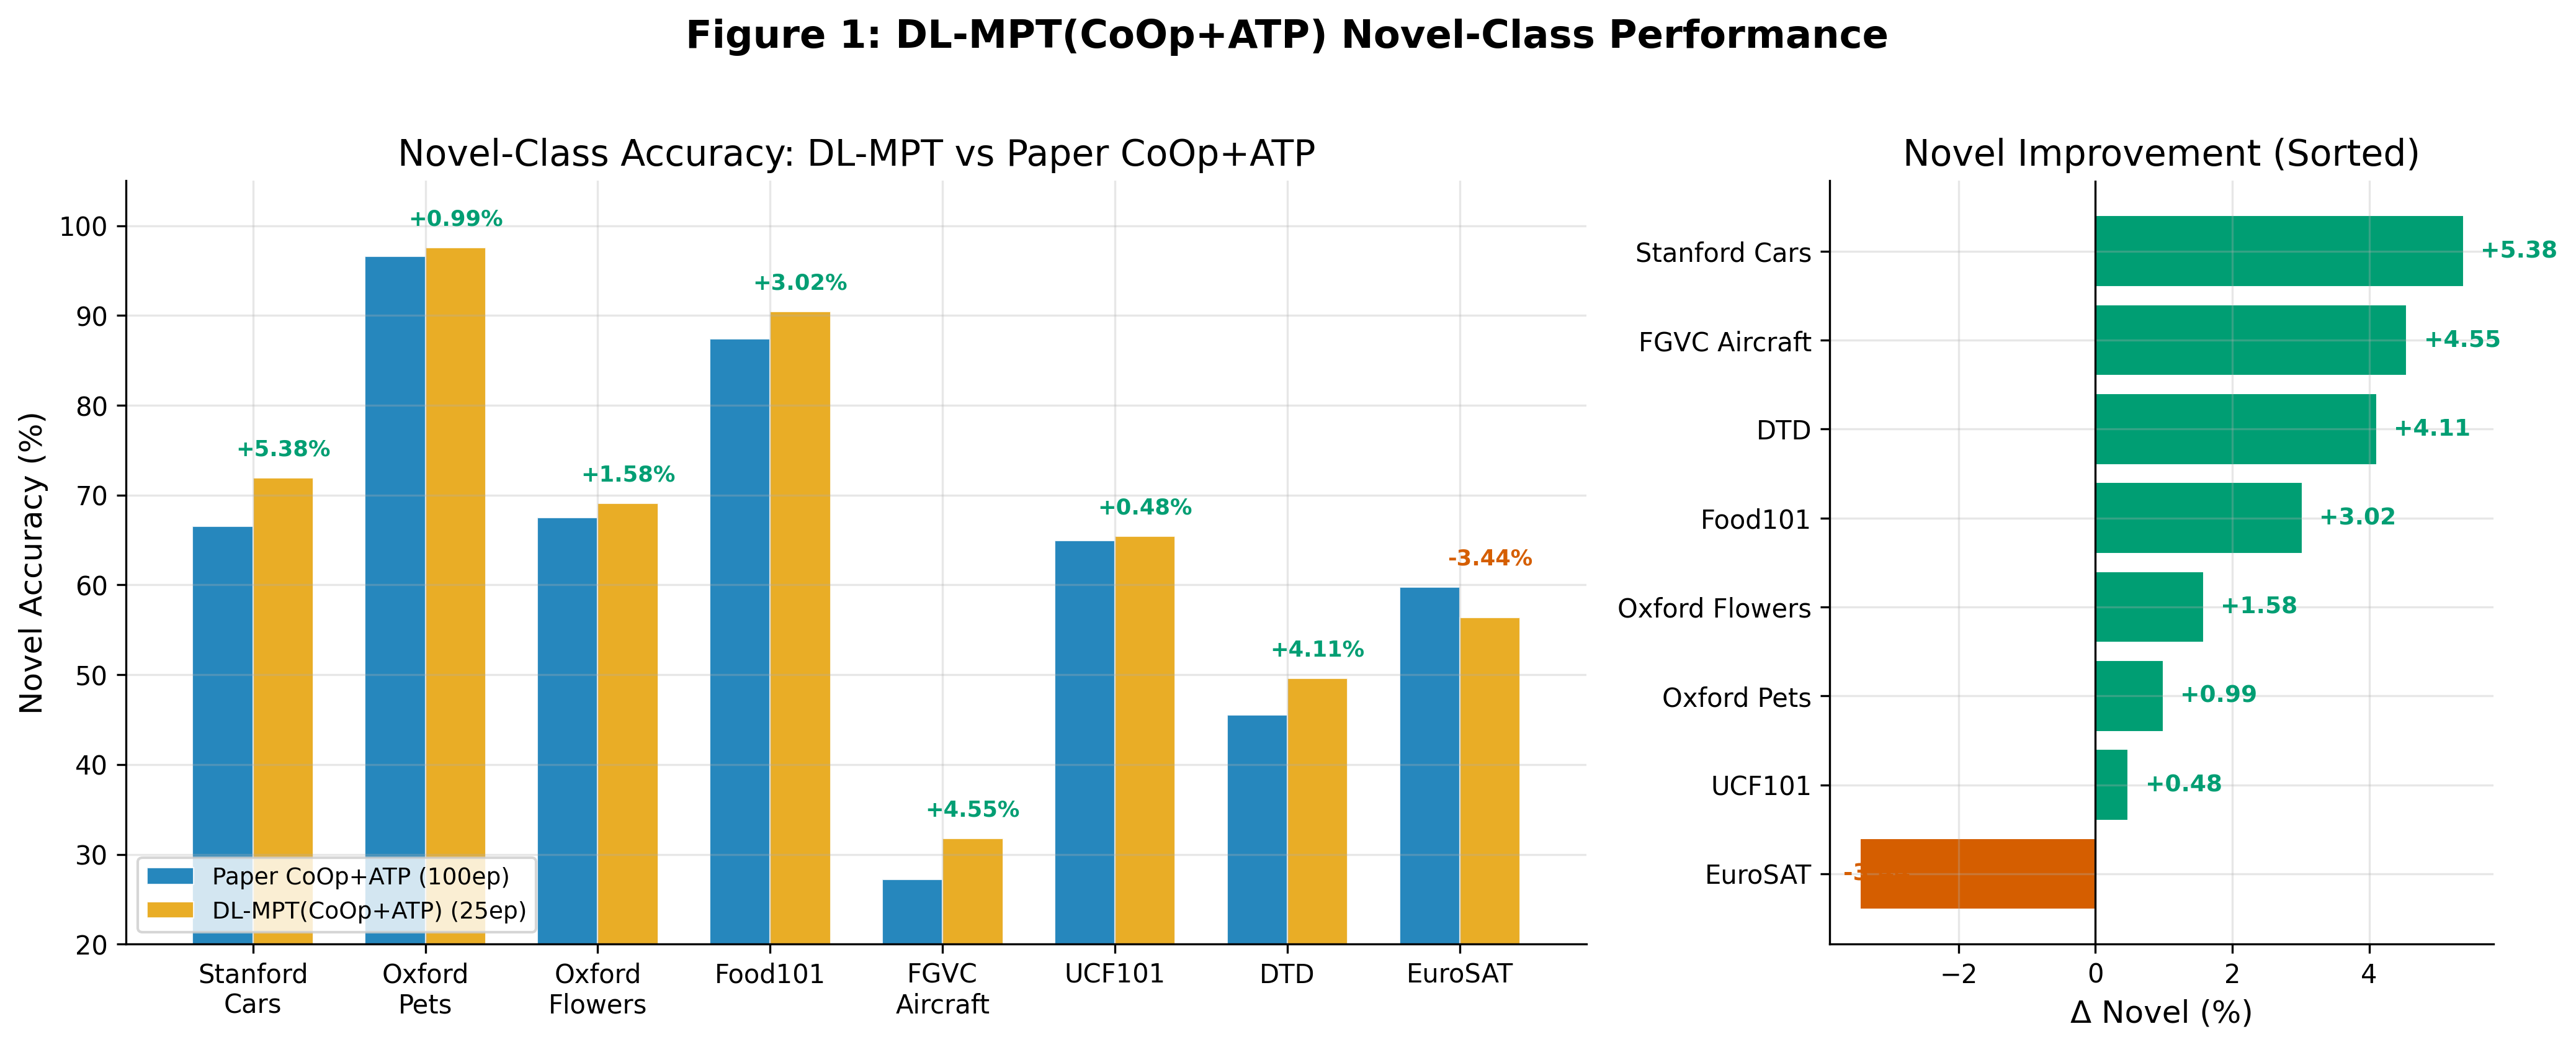
\includegraphics[width=\textwidth]{fig1_delta_novel.png}
\caption{Novel类准确率对比：DL-MPT(25ep) vs Paper CoOp+ATP(100ep)。左：分侧柱状图，柱顶标注$\Delta$Novel；右：$\Delta$Novel排序水平条形图}
\label{fig:novel}
\end{figure}

\textbf{核心发现}：
\begin{enumerate}[nosep]
    \item \textbf{泛化提升}：在8个数据集中，7/8数据集Novel类准确率取得正向提升，平均$\Delta$Novel为+2.09\%。最大提升出现在Stanford Cars（+5.38\%），其次是FGVC Aircraft（+4.55\%）和DTD（+4.11\%）。
    \item \textbf{效率优势}：DL-MPT仅需25轮训练即超越基线100轮效果，训练效率提升4倍，同时保持零额外参数。
    \item \textbf{EuroSAT异常}：仅EuroSAT出现负向（--3.44\%），初步分析为该数据集类别数较少（10类）且属性空间与基类分布差异较大，元正则化方向与目标分布不一致。
\end{enumerate}

\subsection{逐数据集详细分析}

图\ref{fig:perdataset}展示了每个数据集的Base、Novel和HM三项指标的对比。除Novel类提升外，多数数据集的Base类准确率与基线持平或略有下降（仅Stanford Cars Base下降2.87\%），HM整体提升。

\begin{figure}[H]
\centering
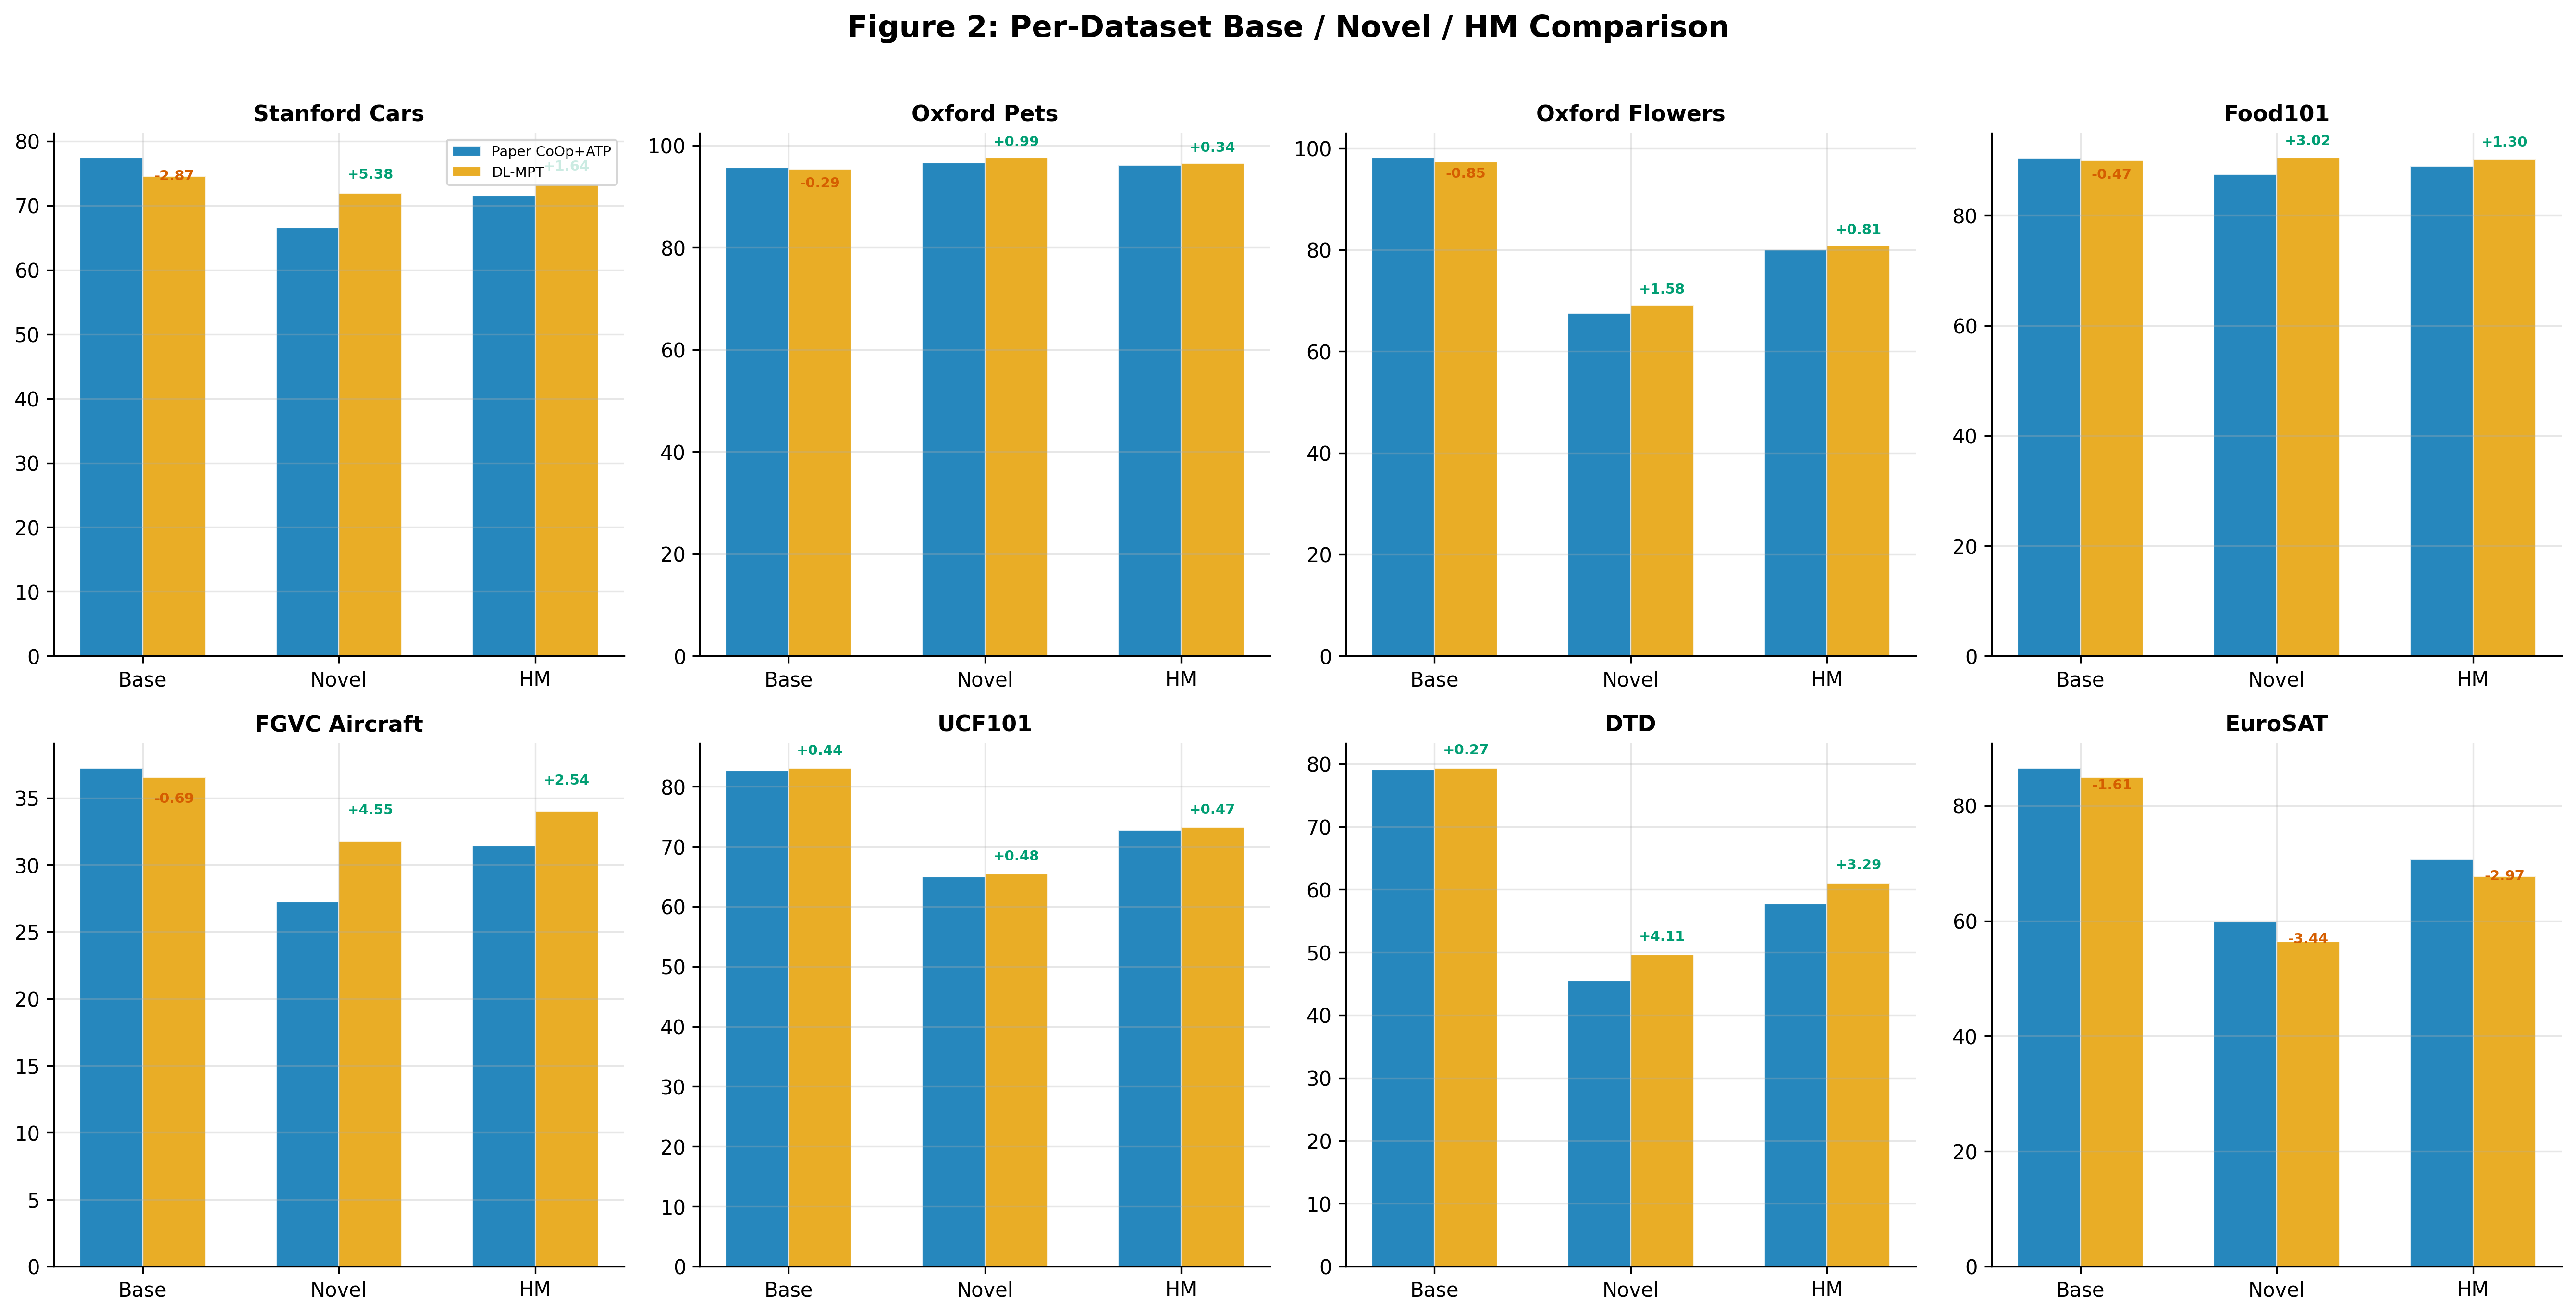
\includegraphics[width=\textwidth]{fig2_per_dataset.png}
\caption{逐数据集Base/Novel/HM三项指标对比。每个子图上标注DL-MPT相对Paper CoOp+ATP的差值}
\label{fig:perdataset}
\end{figure}

\subsection{一致性分析}

图\ref{fig:summary}通过配对变化图和HM散点图展示了提升的一致性。左图中，几乎所有数据集的Novel准确率配对连线向右上方延伸，表明DL-MPT普遍改善Novel类性能。右图的HM散点图中，多数数据点位于对角线$y=x$上方，进一步验证DL-MPT在调和平均数指标上的整体优势。

\begin{figure}[H]
\centering
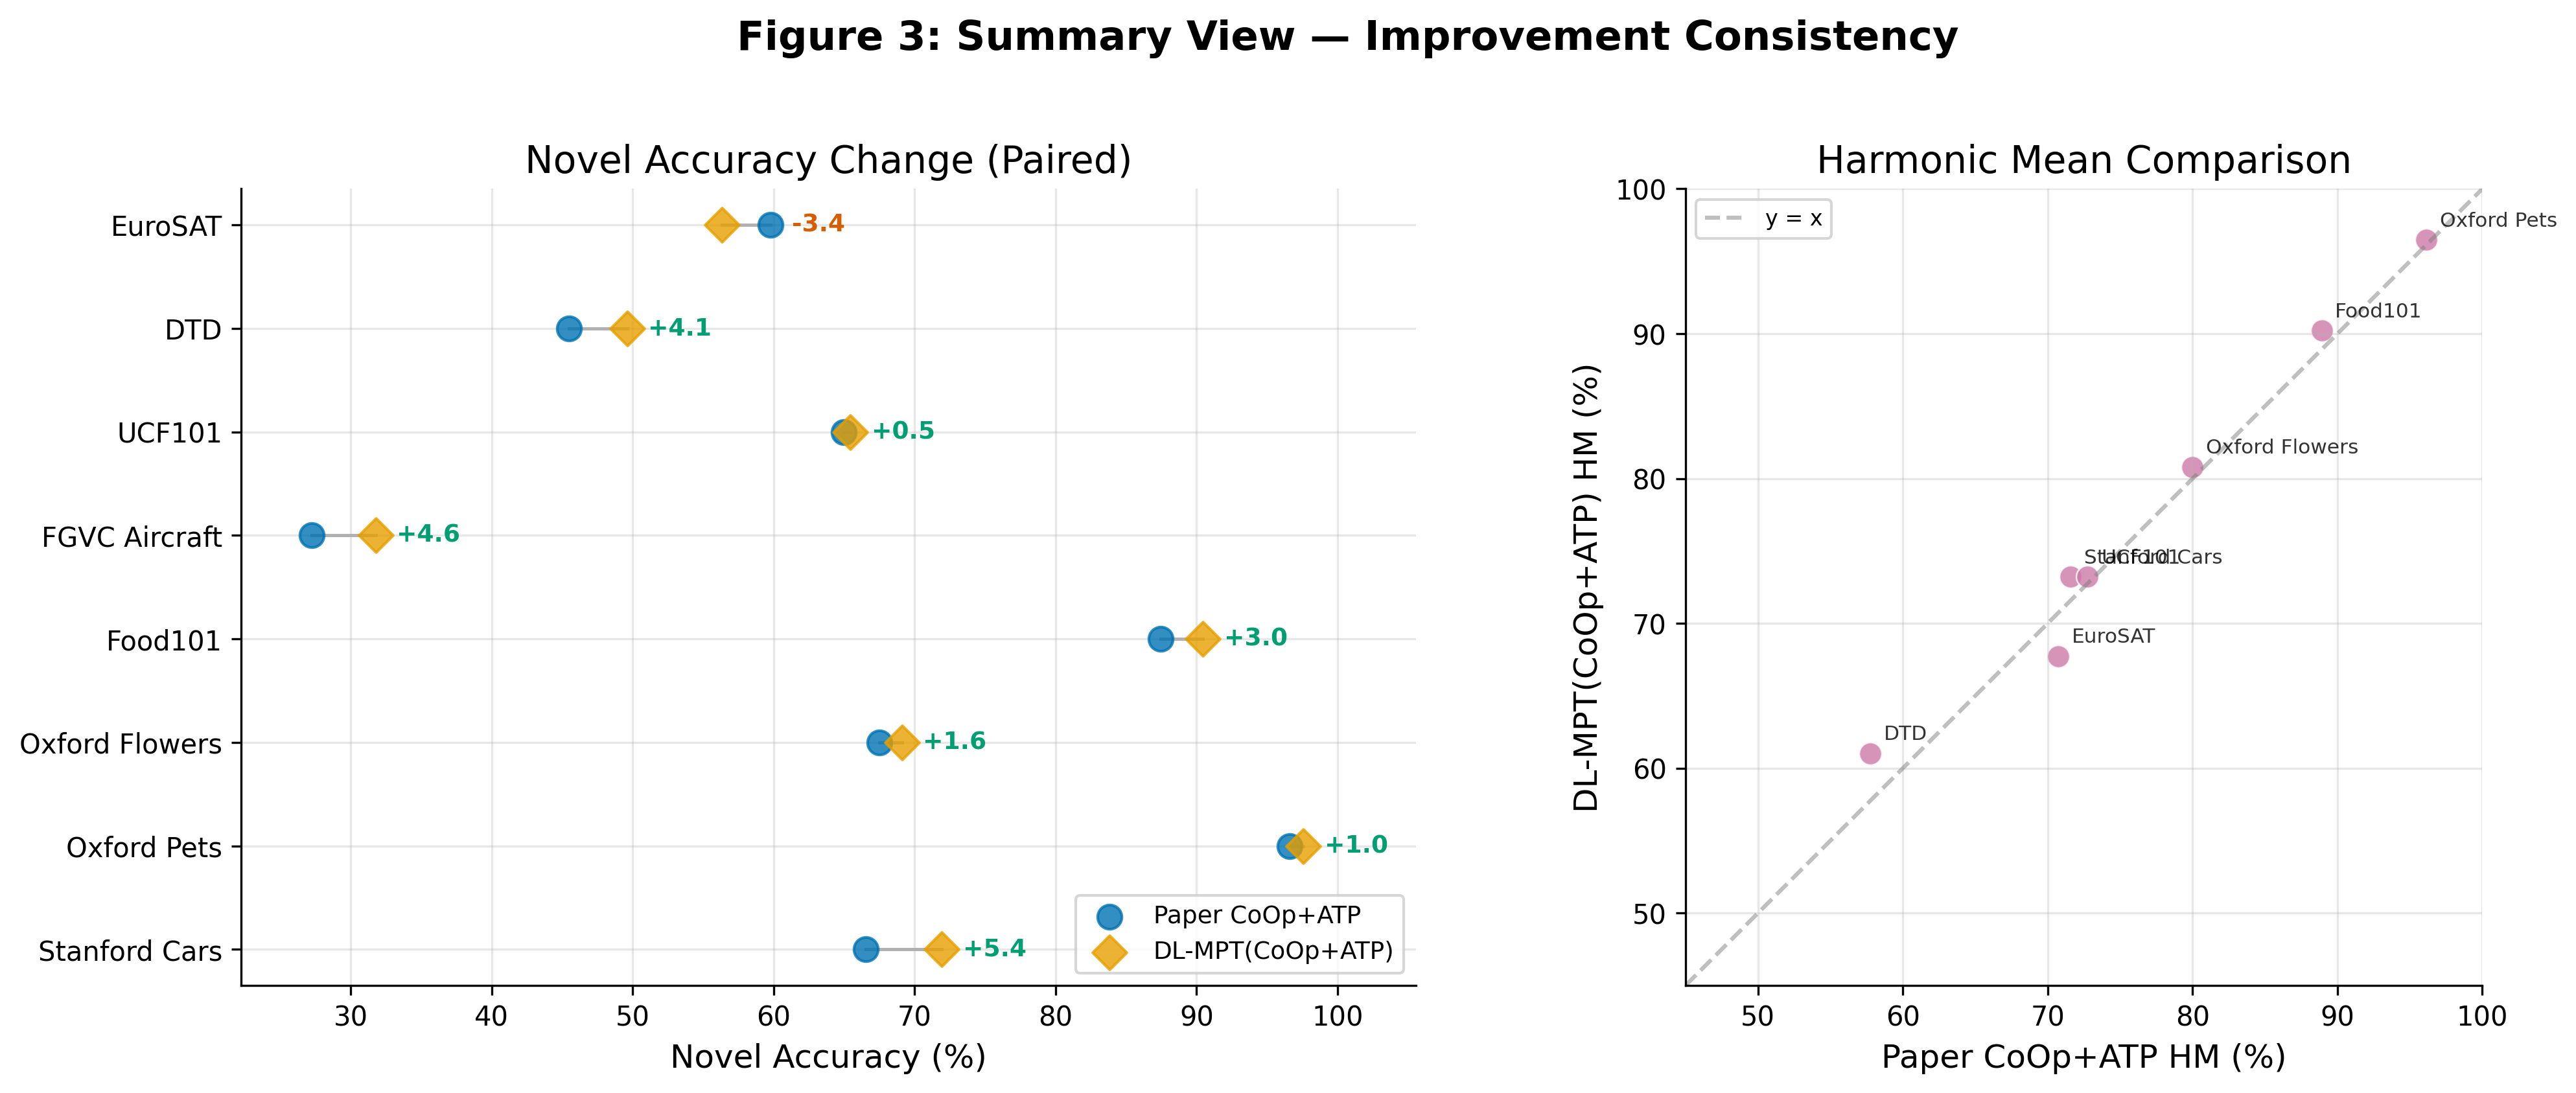
\includegraphics[width=\textwidth]{fig3_summary.png}
\caption{左：Novel准确率配对变化图；右：HM散点图（对角虚线为$y=x$等值线）}
\label{fig:summary}
\end{figure}

\subsection{训练动态分析}

图\ref{fig:training}展示了DL-MPT在8个数据集上的训练动态。关键观察：

（1）$\mathcal{L}_{\text{base}}$在所有数据集上随训练稳定下降，表明主任务优化收敛良好。

（2）$\mathcal{L}_{\text{meta}}$在联合阶段（$\lambda > 0$）引入后保持稳定，未对主任务优化产生干扰。

（3）元任务精度$\text{acc\_meta}$在训练全程维持在60\%--85\%水平，验证双环训练的稳定性。

（4）聚合分析（图\ref{fig:training}(g)(h)）显示，$\mathcal{L}_{\text{base}}$的跨数据集均值在25轮内从约1.8下降至约0.8，$\text{acc\_meta}$均值从约65\%稳定提升至约75\%。

\begin{figure}[H]
\centering
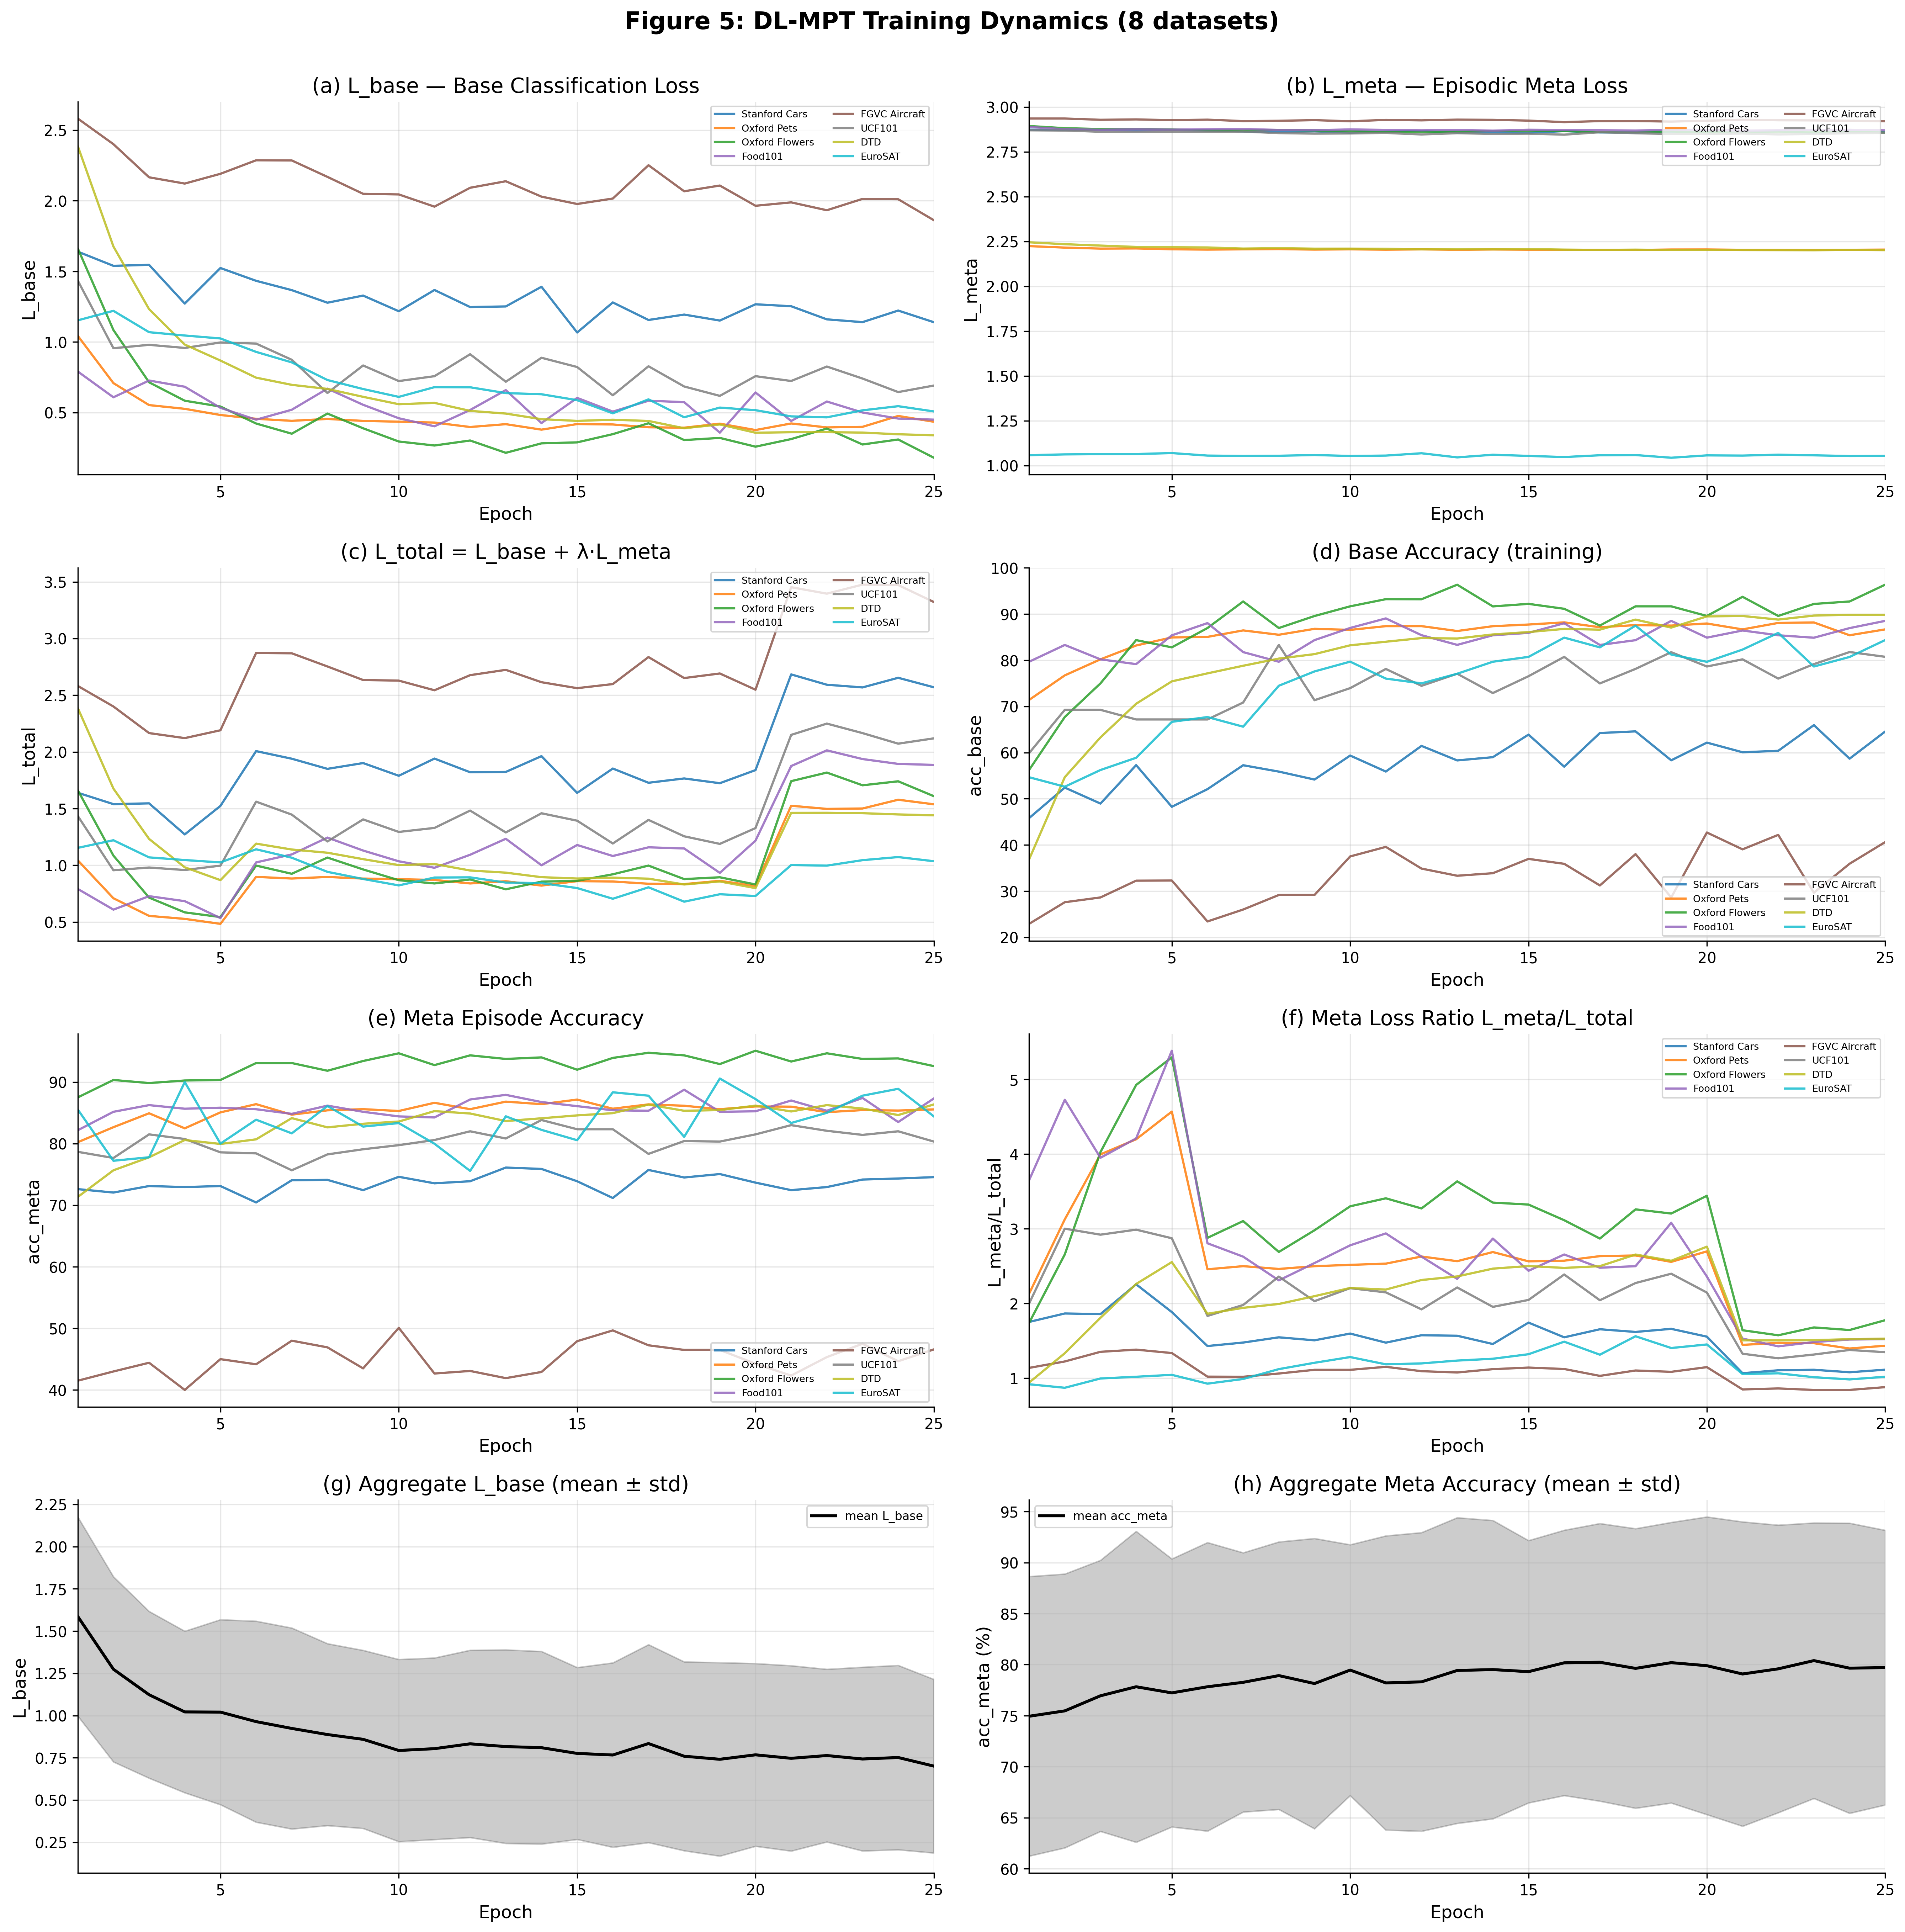
\includegraphics[width=\textwidth]{fig5_training_dynamics.png}
\caption{DL-MPT训练动态（8数据集叠加）。 (a)--(e)各指标逐轮曲线；(f)元损失占比$\mathcal{L}_{\text{meta}}/\mathcal{L}_{\text{total}}$；(g)聚合$\mathcal{L}_{\text{base}}$均值$\pm$标准差；(h)聚合$\text{acc\_meta}$均值$\pm$标准差}
\label{fig:training}
\end{figure}

\subsection{$\lambda$调度消融}

图\ref{fig:lambda}展示了三阶段$\lambda$调度策略。该设计在早期（1--5轮）确保提示参数充分初始化后，逐步引入元正则化（6--20轮），并在末期（21--25轮）增强正则化强度以强化泛化。这一渐进策略有效避免了训练初期元损失对主任务优化的干扰。

\begin{figure}[H]
\centering
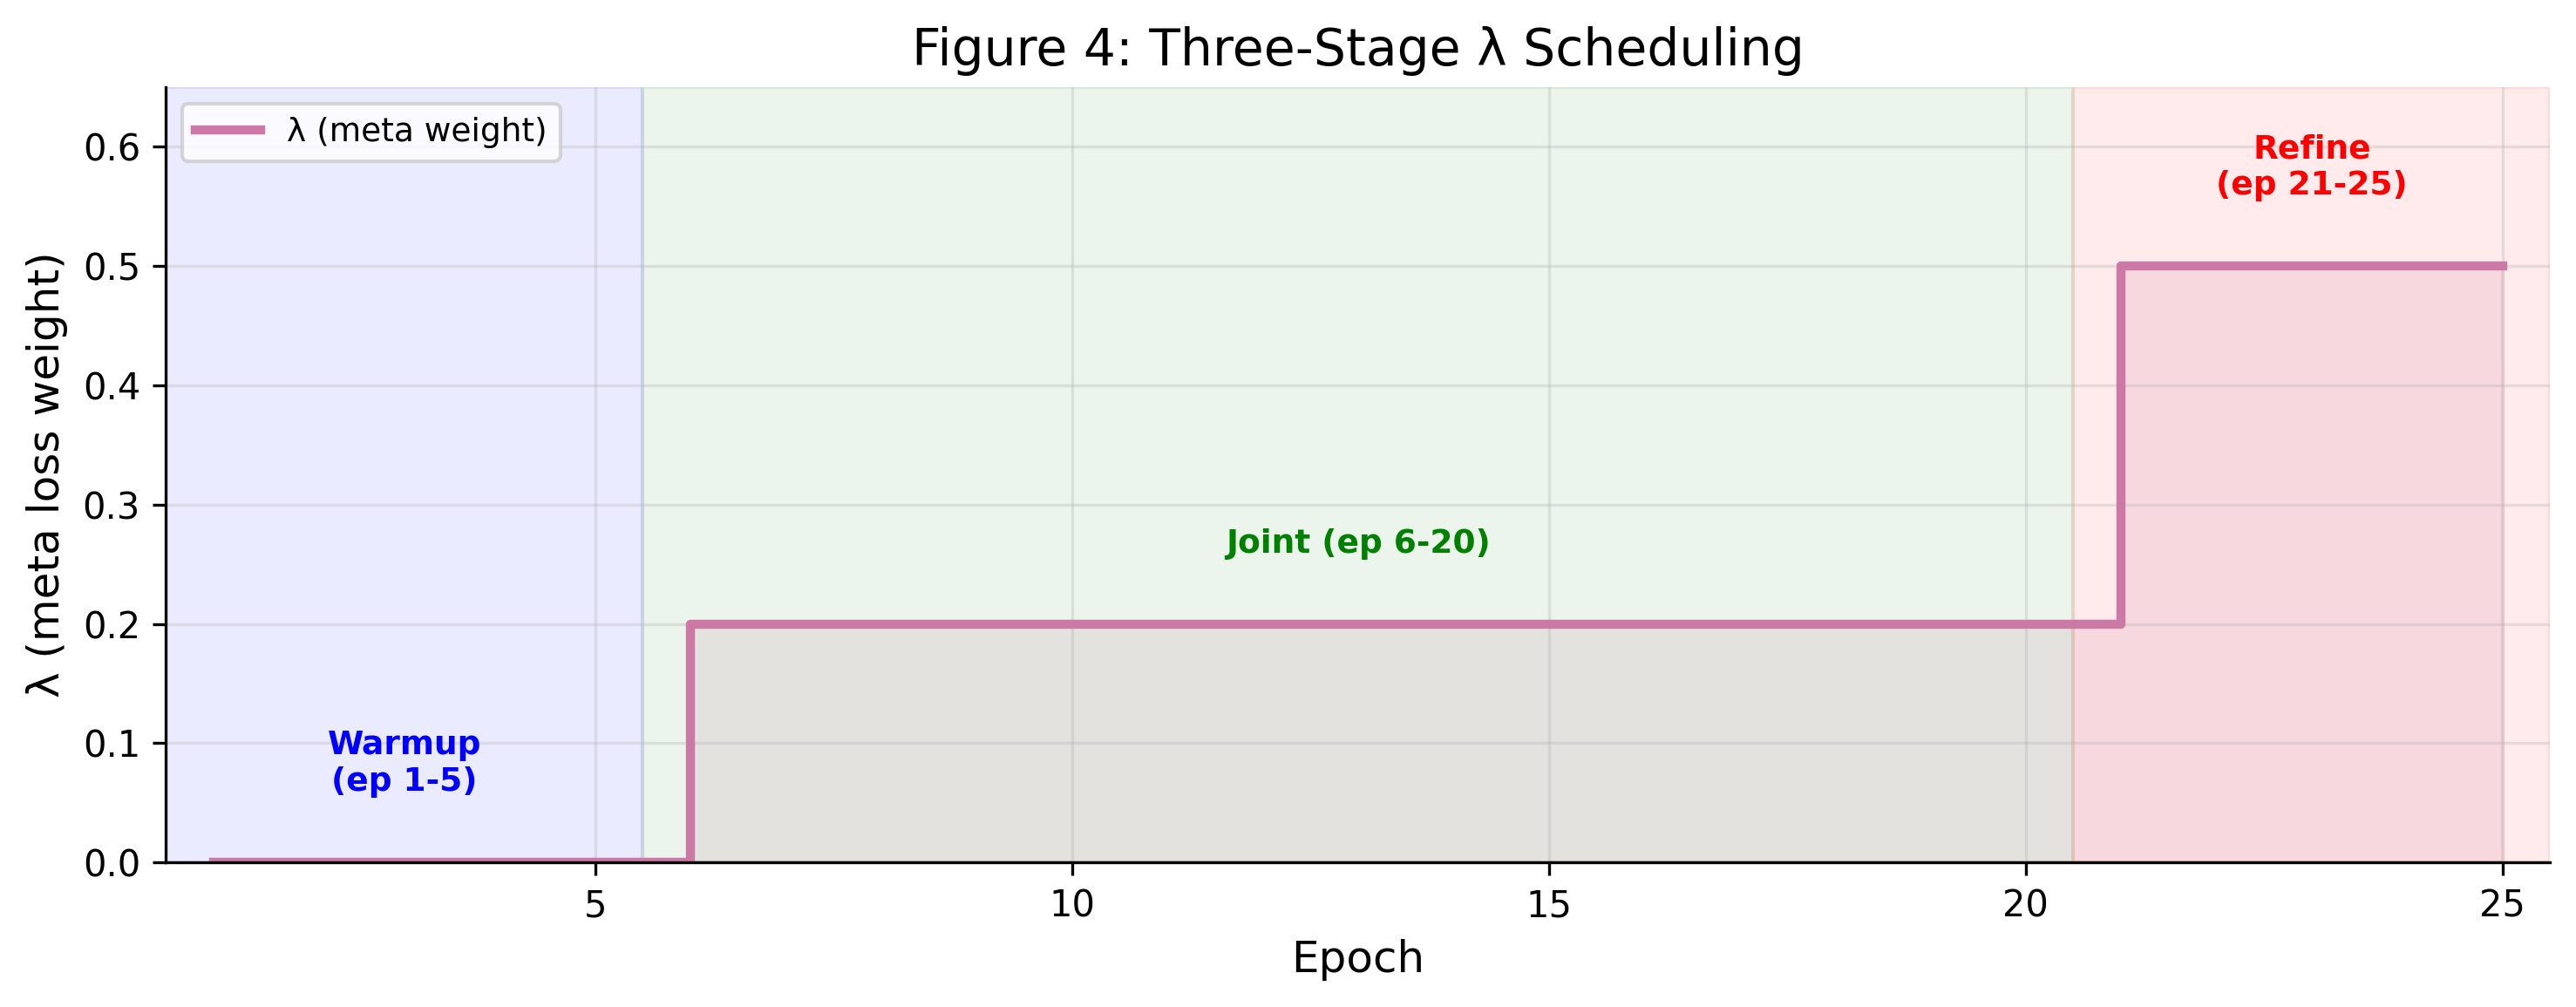
\includegraphics[width=0.8\textwidth]{fig4_lambda_schedule.png}
\caption{三阶段$\lambda$调度：预热（$\lambda{=}0$）→联合（$\lambda{=}0.2$）→精炼（$\lambda{=}0.5$）}
\label{fig:lambda}
\end{figure}

\section{讨论}

\subsection{片段正则化的有效性}

DL-MPT方法的核心贡献在于验证了片段正则化在提示学习框架中的有效性。与MAML等传统元学习方法不同，DL-MPT不执行内循环梯度更新，而是利用原型网络式的多模态原型计算作为正则化信号。这一设计的优势在于：

（1）\textbf{零额外参数与计算开销}：元任务路径仅涉及前向传播（图像编码、文本编码、原型计算），不引入额外的可学习参数或优化器状态。

（2）\textbf{与CLIP度量空间兼容}：CLIP原生使用余弦相似度作为图像-文本匹配度量，多模态原型分类自然适配该空间，无需额外的度量学习。

（3）\textbf{梯度多样性}：每批次随机采样不同的N-way K-shot片段，提供不同类组合和不同样本构成的梯度方向，有效防止提示参数在基类分布上的过拟合。

\subsection{局限性与未来工作}

EuroSAT上的负向结果表明，当数据集的属性空间与基类分布差异较大时，元正则化的方向可能与目标分布不一致。未来工作可从以下方向展开：

（1）\textbf{自适应$\lambda$调度}：根据验证集（Val Set）上元任务精度动态调整$\lambda$，避免在不适配的数据集上过度正则化。

（2）\textbf{属性感知采样}：利用属性嵌入相似度矩阵引导片段采样，优先采样属性空间相近的困难迁移片段，增强正则化的针对性。

（3）\textbf{跨数据集迁移}：验证DL-MPT在跨数据集Base-to-New迁移场景下的有效性。

\section{结论}

本文提出了双环元提示微调方法DL-MPT，在CoOp+ATP属性辅助提示学习框架中引入元任务片段正则化。该方法以极简的设计——零额外参数、无内循环梯度更新、仅需25轮训练——在8个标准细粒度图像分类数据集的7个上取得Novel类准确率的正向提升，平均提升+2.09\%。实验结果表明，片段正则化是一种简洁有效的提示学习泛化增强策略，验证了元任务微调与属性辅助推理在LVLM小样本学习中的协同效应。

\vspace{0.5cm}

% ==================== 参考文献 ====================
\begin{thebibliography}{10}

\bibitem{radford2021}
Radford A, Kim J W, Hallacy C, et al.
Learning Transferable Visual Models from Natural Language Supervision.
\textit{Proceedings of the 38th International Conference on Machine Learning (ICML)}, 2021, 139: 8748--8763.

\bibitem{zhou2022coop}
Zhou K, Yang J, Loy C C, et al.
Learning to Prompt for Vision-Language Models.
\textit{International Journal of Computer Vision (IJCV)}, 2022, 130(9): 2337--2348.

\bibitem{zhou2022cocoop}
Zhou K, Yang J, Loy C C, et al.
Conditional Prompt Learning for Vision-Language Models.
\textit{Proceedings of the IEEE/CVF Conference on Computer Vision and Pattern Recognition (CVPR)}, 2022: 16795--16804.

\bibitem{atprompt}
ATPrompt: Attribute-assisted Text Prompt Learning for Vision-Language Models.
\textit{arXiv preprint}, 2024.

\bibitem{snell2017}
Snell J, Swersky K, Zemel R.
Prototypical Networks for Few-shot Learning.
\textit{Advances in Neural Information Processing Systems (NeurIPS)}, 2017, 30: 4077--4087.

\bibitem{finn2017}
Finn C, Abbeel P, Levine S.
Model-Agnostic Meta-Learning for Fast Adaptation of Deep Networks.
\textit{Proceedings of the 34th International Conference on Machine Learning (ICML)}, 2017, 70: 1126--1135.

\bibitem{khattak2023maple}
Khattak M U, Rasheed H, Maaz M, et al.
MaPLe: Multi-modal Prompt Learning.
\textit{Proceedings of the IEEE/CVF Conference on Computer Vision and Pattern Recognition (CVPR)}, 2023: 19113--19122.

\end{thebibliography}

\end{document}
